% !TEX root=../thesis.tex

\chapter{Preliminary}
\section{Deep Learning}
Deep learning is a state-of-art machine learning algorithm that implements the concept of neural network.
It trains a model designed for a specific task (hence discriminative) while simultaneously learns the feature representations in an unsupervised manner. 
As will be explained in detail later in this chapter, the parameters in each layer are learned using Stochastic Gradient Descent (SGD) \cite{bottou2010large}, while the gradients are back-propagated from the top layer down to the input data.

CNN (Convolutional Neural Network) is a subgroup of deep learning model intended to emulate the visual cortex of animals. 
Compared with other neural network structures, CNN is characterized by its sparse local spatial connectivity between adjacent layers. 
This means each hidden unit in layer $ m $ is connected only with a subset of units in layer $ m-1 $ that have spatially contiguous \textit{receptive field}
\cite{cnnlenet} (illustrated in \autoref{fig:cnnsparse}). 
Here, receptive field is a term borrowed from biological visual perception referring to the sub-region on visual field a neuron is sensitive to.

\begin{figure}[h]
\centering
\begin{tikzpicture}
[>=stealth, nodes={draw, circle}, level distance=10mm]
\node (y) {} 
child [sibling distance=10mm]{ node {}
child {node {}}
child {node {}}
}
child [sibling distance=10mm]{ node (n) {}
child {node {}}
child {node (2) {}}
};
\node[right=of n, xshift=5mm] (x) {} [sibling distance=10mm]
child {node (1) {}}
child {node {}};
\draw[shorten <= 1mm,shorten >= 1mm, dotted] (1) -- (2);
\draw (x) -- node[cross out,draw=red]{} (y);
\end{tikzpicture}
\caption[Sparse connectivity in CNN]{Units of two consecutive layers are only connected if their receptive field is spatially contiguous.}\label{fig:cnnsparse}
\end{figure}
\subsection{Fundamental Components in a CNN}
A CNN typically comprises of 5 kinds of layers. These layers, equivalent to neurons in a classic neural network, perform a series of linear and non-linear operations on the input image. The output of these layers is called \textit{feature map}.
\subsubsection{Convolutional Layer}\label{sec:cnnlayers}
Convolutional layer is the core of a CNN. It applies a linear shift-invariant filter, called \textit{kernel} on the input feature.
\autoref{fig:convkernel} (source \cite{iosconvolution}) illustrates a convolutional operation with a $ 3\times3 $ kernel on a single input channel. This operation is repeated over the whole spatial dimensions as well as all input channels. 
Mathematically, we can write a 2D convolution on input $ \x $ with kernel $ \w $ at point $ (w, h) $ as
\[ \w \ast \x(w,h) =  \sum_{q=-\frac{1}{2}(c-1)}^{\frac{1}{2}(c-1)}\sum_{p=-\frac{1}{2}(c-1)}^{\frac{1}{2}(c-1)}\w(p,q)\x(w-p,h-q), \]
where $ c $ denotes the kernel size.

\begin{figure}[h]
\centering
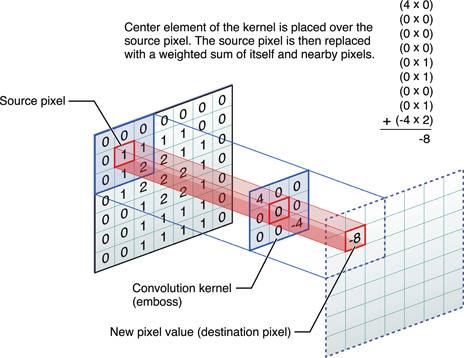
\includegraphics[width=0.5\linewidth]{figures/kernel_convolution.jpg}
\caption[Illustration of 2D convolution]{Illustration of a 2D convolutional operation using a single kernel of size 3 on a input layer}\label{fig:convkernel}
\end{figure}
A convolutional kernel is associated with each input channel and each output channel. Formally, given a input feature map $ \x$, the $ k' $-th channel in output can be expressed as
\[ h[w, h, k'] = b_{k'} + \sum_{k\in K_{in}}\x[w,h,k]\ast\w_{k'k}. \]
$\mathbf{b} $ and $ \w $ together make up $ K'\times K\times c\times c $ parameters for a convolutional layer. 

Since the values of each kernel $ \w_k $ stay unchanged over the whole feature map, the total number of parameters are greatly reduced. This improves the learning efficiency as well as the generalization property of the network. Meanwhile it also undertones that the local response to a pattern is independent of its spatial location.
\subsubsection{Pooling Layer}
Pooling layers are used to aggregate input feature in a region to reduce its dimension. Furthermore, since small translation or perturbation in the input within the pooling region does not affect the output, pooling also introduces certain degree of translation-invariance.

The pooling operation is parameterized by stride and kernel size. An example of a MaxPooling is illustrated in \autoref{fig:maxpool} (source \cite{standfordonline}).
\begin{figure}[h]
\centering
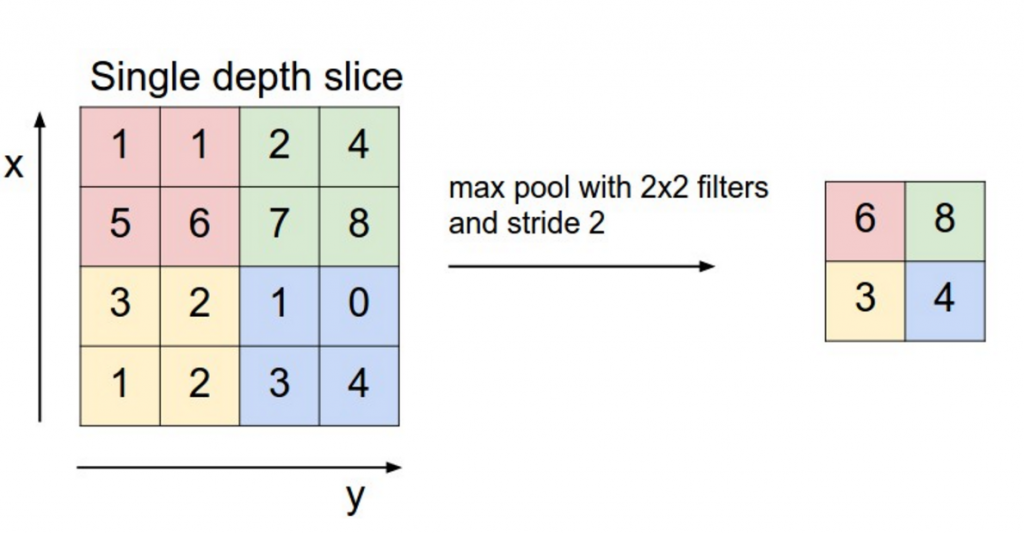
\includegraphics[width=0.5\linewidth]{figures/maxpooling.png}
\caption[Illustration of MaxPooling]{Illustration of a MaxPooling operation with kernel size 2 and stride 2}\label{fig:maxpool}
\end{figure}
\subsubsection{Rectified Linear Unit Layer}
Rectified Linear Unit (ReLU) layer is one of the activation functions that simulate switches in neurons by performing a fixed non-linear operation on the input signal.

ReLu performs a simple threshold \[ f(x) = \max(x, 0). \]
Compared to other activation functions, such as $ sigmoid $ and $ tanh $, ReLU exhibits better qualities in accelerating the convergence rate \cite{krizhevsky2012imagenet} and leads to better results \cite{maas2013rectifier}.
\subsubsection{Fully Connected Layer}
Fully connected layer, also known as inner product layer, performs an inner product between weight vector $ \left\lbrace w_k \right\rbrace_{1}^{K'} $ and all channels of the input data. Given an input $ \x $ of size $ K\times H\times W $, the output is a vector of length $ K' $, whose value at position $ k' $ is
\[ \mathbf{h}[k'] = b_{k'} + \sum_{w, h, k}\x[w,h,k]\w_{k'}[w,h,k]. \]
As a result, fully connected layers have $ K' \times K\times H\times W  $ parameters.
\subsubsection{DropOut Layer}
DropOut \cite{hinton2012improving} is a recent invention in deep learning. 
It addresses the issue of overfitting by randomly dropping, i.e. zero-setting, features together with their connections in training. 
Intuitively, this forces the units to be independent of each other and hence prevent units from excessive co-adapting.

During training a unit is dropped with probability $ q $ (\textit{dropout rate}), i.e.
\[ f(x) = \begin{cases}
0, \; \mathrm{if}\, p \le q \\
x, \; \mathrm{otherwise}
\end{cases}. \]
The resulting feature is then multiplied by a factor of $ \frac{1}{q} $ to preserve the scale of output (thus also input of the upper next layer), which is particularly important in fine-tuning an pre-trained model.

Dropout proves to be very effective for tasks that inhabit dense input features and outperforms conventional methods tackling this issue, such as $ L1 $ or $ L2 $ weight penalties \cite{srivastava2014dropout}.
\subsection{Parameter Learning via Back-propagation}
Training a deep neural network, supervised or not, works by optimizing a target function.

For an supervised $ K $-class classification problem with labeled data $ \mathcal{X} =  \lbrace\x_i, \hat{y}_i \rbrace_{i=0}^{N} $ and predictions $\lbrace y_i \rbrace_{i=0}^{N} $, this target function is often defined as the softmax loss:
\begin{align}
L(\w; \mathcal{X}) &= \dfrac{1}{N}\sum_{i=0}^{N-1} L(\w; \x_i, y_i)\nonumber\\
& = -\dfrac{1}{N}\sum_{i=0}^{N-1}\log \Pr(y_i = \hat{y}_i |\x_i, \w)\label{eq:softmaxloss} \\
& = -\dfrac{1}{N}\sum_{i=0}^{N-1}\sum_{j=0}^{K-1}\lbrace \hat{y}_i = j \rbrace\log p_{y|x}(j|\x_i, \w)\nonumber, 
\end{align}
where $ \lbrace \hat{y}_i = j \rbrace $ is the indicator function that equals $ 1 $ when the predicate is true, namely:
\[ \lbrace \hat{y}_i = j \rbrace = \begin{cases}
1 & \text{if $ \hat{y}_i = j $}\\
0 & \text{otherwise}
\end{cases} .\]
$ p_{y|x}( j|\x_i, \w) $, the probability that $ \x_i $  is classified as $ j $, is computed with softmax function:
\[ p_{y|x}(j|\x_i, \w) = \dfrac{\exp h_j\left(\x,\w\right) }{ \sum_{j=0}^{K-1}\exp h_j\left(\x,\w\right)}, \]
where $ h_j\left(\x,\w\right) $ denotes the classification score of $ \x_i $ for class $ j $ computed by the network.

The objective of training a network is to find the parameters $ \w $ that minimize the softmax loss, i.e. 
\[ \w = \argmax L(\w; \mathcal{X}). \]

\paragraph{Stochastic Gradient Descent}
In Deep Learning, this optimization problem is solved using the idea of \textit{gradient descent}. Gradient descent is a simple learning algorithm that updates the parameters $ \w $ iteratively along the direction that induces the steepest descend in $ L $, which is effectively the negative gradient of $ L $ wrt $ \w $. 
The magnitude of update is determined by a hyperparameter \textit{learning rate} $ \eta $. Formally, the parameter update at step $ t $ can be written as
\[ \w_{t+1} = \w_{t} - \eta\derivative{L}{\w}. \]
The gradient, computed as \[ \dfrac{1}{N}\sum_{i=0}^{N-1} \derivative{L(\w; \x_i, y_i)}{\w}, \] is very expensive to evaluate over the whole data samples, hence it is often approximated with a subset of samples (called \textit{batch}) $ \lbrace \x_m, y_m \rbrace_{m=0}^{M} $, where $ M \leq N$ denotes the number of samples in a batch, also referred to as \textit{batchsize}. In other words, 
\[ \derivative{L}{\w} = \dfrac{1}{M}\sum_{m=0}^{M}\derivative{L(\w; \x_m, y_m)}{\w}. \]
The approximation formulates an important variant of gradient descent, namely \textit{stochastic gradient descent} (SGD). 

Furthermore, to improve the convergence rate and stability of the algorithm, instead of using the gradient as update value only, the parameters are updated with a linear combination of the gradient and the previous update value $ \v_{t} $, i.e. 
\begin{align}\label{eq:sgd}
\v_{t+1} & = \mu \v_{t} - \eta \derivative{L}{\w}\\
\w_{t+1} & = \w_{t} +  \v_{t+1}.
\end{align}
By doing so, each update is smoothened across previous iterations, which pushes the parameters towards the global minimum even under oscillating gradients \cite{polyak1964some}. The hyperparameter $ \mu $ is called \textit{Momentum}, it indicates the amount of influence from the previous iterations and effectively increases the magnitude of update.

SGD is the most basic yet most commonly used policy for parameter learning, while several variations exist that improve this general form with different focus (e.g. Adaptive Gradient \cite{duchi2011adaptive} and Adaptive Momentum \cite{kingma2014adam}).

\paragraph{Backpropagation}
In deep learning, the mapping from input $ \x $ to the final output $ y $ is composed of many layers of linear and non-linear functions. 
In order to calculate the $ \derivative{L}{\w} $ in \autoref{eq:sgd}, one needs to apply the chainrule in basic calculus.
If $ y=f\left(h\right) $, while $ h $ is a function of $ x $, i.e. $ y = f\circ h\left(x\right) $, chainrule gives the following formula to compute the derivative $ \derivative{y}{x} $:
\[ \derivative{y}{x} =  \derivative{f}{h}\derivative{h}{x}.\]
Essentially \textit{Backpropagation} is nothing else but applying chainrule sequentially top-to-down from the final loss layer to compute the gradients of the loss function w.r.t. all parameters.

Assume we know the gradient of loss function $ L $ wrt to the input feature map of $ l $-layer $ \derivative{L}{\x_l} $,
where $ \x_l $ is computed from layer $ l-1 $ 
\[ \mathbf{x}_l = h_{l-1}\left(\x_{l-1}, \w_{l-1}\right). \]
We can easily calculate two partial derivatives
\begin{equation}\label{eq:backprop}
\derivative{L}{\w_{l-1}} = \derivative{L}{\x_l}\derivative{h_{l-1}}{\w_{l-1}} ,\quad
\derivative{L}{\x_{l-1}} = \derivative{L}{\x_l}\derivative{h_{l-1}}{\x_{l-1}}.
\end{equation}
 We refer the two derivatives as \textit{param derivatives} and \textit{data derivatives}. While the former is the desired gradient in \autoref{eq:sgd}, the latter is propagated down to the lower layers, where this process will be repeated to compute all remaining param derivatives.

To summarize, during backpropagation each layer of the network takes the data derivatives from the upper layer, computes param derivatives and data derivatives using \autoref{eq:backprop} and outputs data derivatives to the lower layers. 
%\begin{table}
%	\centering
%	\begin{tabular}{r|c|c}
%& $ \derivative{L}{\w} $ & $ \derivative{L}{\x} $\\ \hline
%& $ \derivative{L}{\w} $ & $ \derivative{L}{\x} $\\ \hline
%\end{tabular}
%\end{table}
\subsection{Feature Map}\label{sec:featmap}
Feature map refers to the output of a convolutional layer (typically after activation layer such as ReLu).
As this naming indicates, a feature map conveys two pieces of information, namely:
\begin{enumerate}
\item what is the feature, encoded in the actual values or activation state of each specific channel in the feature map
\item where is the feature, encoded in the spatial location of an activation.
\end{enumerate}

As is revealed in \cite{zeiler2014visualizing}, each channel of a feature map represents a particular pattern. 
An activation in a specific channel at a specific location essentially describes the existence of a type of pattern at the corresponding location in the input image.
In lower layers, the encoded patterns are usually comprised of low level features, such as edges and corners. 
As one proceeds deeper in the network, they become more abstract and discriminative.
In an object classification model trained for ImageNet, the feature map in the last convolutional layer can be interpreted as representations of different object classes. 

A very explanatory example (shown in \autoref{fig:featuremap}) is given by \cite{kaiminghe}, where the relation between channel, pattern and location is comprehensively illustrated.

\begin{figure}[ht]
\centering
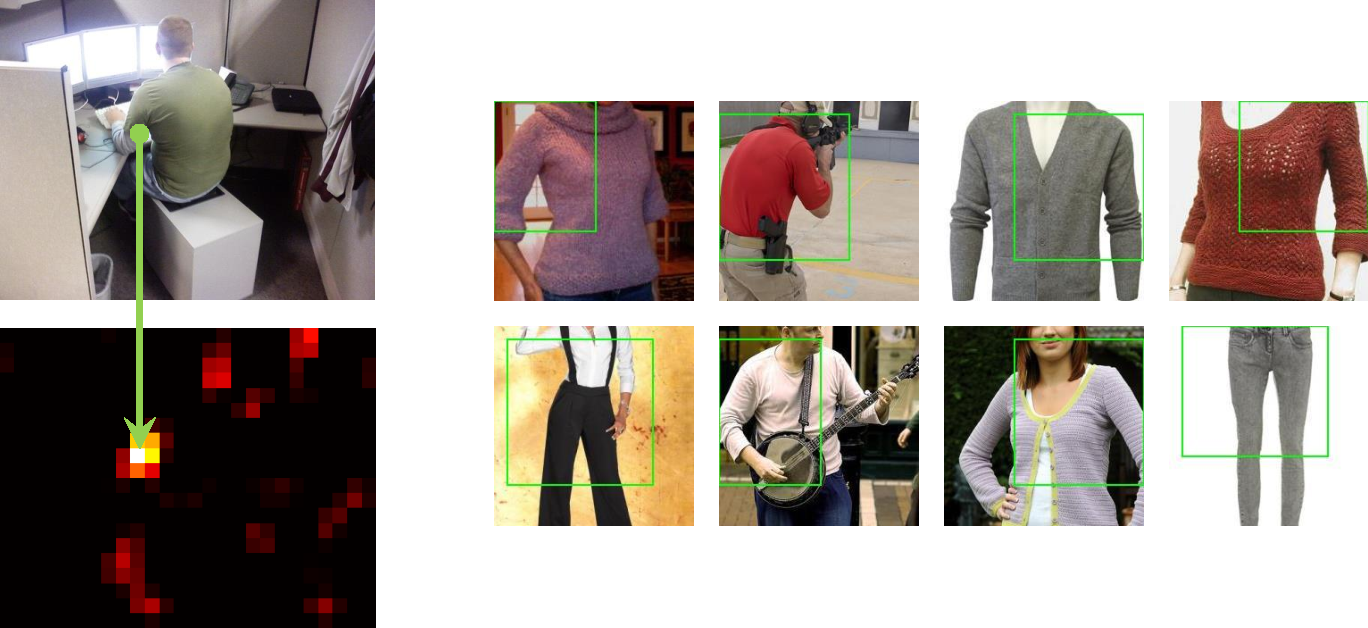
\includegraphics[width=0.9\linewidth]{figures/featuremap.pdf}
\caption[Feature map]{Left: the $ 66 $-th channel of a sample feature map in conv5 layer. Right: Other image samples that generate high response in this channel. Simply put, a high response in this channel indicates there is a "$ \lambda $" shaped object at the corresponding position in input image.}\label{fig:featuremap}
\end{figure}

Moreover, as is pointed out by \cite{kaiminghe}, while the spatial position explicitly encodes the location of a given pattern, the feature value itself also provides \textit{finer} position information.
This is concluded from the fact that from the visualization of a single activation one can extract the "outline" of the targeted pattern (see \autoref{fig:singleresponse} given by \cite{zeiler2014visualizing}).
As a result, one can utilize the feature values across all channels to obtain refined localization information of a composed object.

\begin{figure}[ht]
\centering
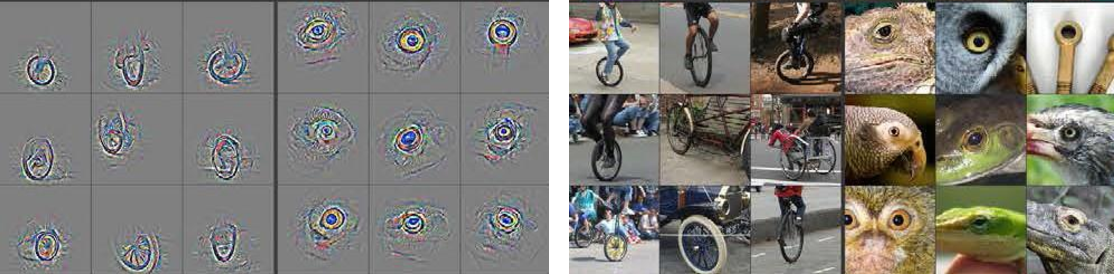
\includegraphics[width=0.8\linewidth]{figures/singleresponse.pdf}
\caption[Single response visualization]{Reconstruction from a single activation from two different channels in conv5 feature map (left) and the corresponding input pattern (right). Reconstructions from the same channel shows subtle differences in outline, implying that the activation value conveys refined locational information.}\label{fig:singleresponse}
\end{figure}

To summarize, both classification and localization information are present in feature maps; while the former is expressed in the activated feature values itself, the latter is encoded in both the feature values and the spatial position of activations.

\section{Dynamic Programming}\label{sec:dp}
Dynamic Programming is a powerful optimization algorithm. Applicable in both discrete and continuous, deterministic and stochastic domains, it is a tool for many complex real-world problems.
In our thesis, we use its finite discrete deterministic form to find the actual action performer from raw person detections.

Discrete deterministic Dynamic Programming constitutes the following problem setup:
\begin{itemize}
\item given the dynamics of a deterministic discrete time (in-)variant system defined in a finite time steps $ N $
\[ \x_{n+1}=f_{n}\left(x_{n}, u_{n}\right) \; \text{with } x_{n} \in \mathcal{X}_{n},\, u_{n}\in \mathcal{U}_{n},\,n\in\lbrace0,1,\dots N-1\rbrace, \]
where $\mathcal{X}_{n} $ and $ \mathcal{U}_{n} $ denote the set of possible state and control input at time $ n $;
\item given the cost of applying input $ u_{n} $ on state $ x_{n} $ at time step $ n $\[ g_{n}\left(x_{n}, u_{n}\right) \]
\item find the optimal policy $ \pi^* $ such that 
\begin{align}
\pi^* &= \argmin J \nonumber\\
&= \argmin_{\pi}\sum_{n=0}^{N}g_{n}\left(x_{n}, u_{n}\right)+g_{T}\left(x_{N},T\right)\nonumber\\
&= \argmin_{\lbrace\mu_{0},\mu_{0},\dots, \mu_{N-1}\rbrace }\sum_{n=0}^{N}g_{n}\left(x_{n}, \mu_{n}\left(x_n\right)\right)+g_{N}\left(x_{N}\right)\label{eq:objective}
\end{align}
where $ \mu_{n} $ is a state dependent single step time-(in)variant strategy $ u_{n} = \mu_{n}\left(x_{n}\right)$. 
Notice although system dynamics does not appear in \autoref{eq:objective}, it is integrated with the time increment.
\end{itemize}

Directly solving \autoref{eq:objective} would require evaluation of all possible connections. 
For a fully connected system (every state in the current step is reachable from every state in the previous step), if the average number of states in a stage is $ K $, the computations complexity would be $ \mathcal{O}\left(K^N\right) $.

Dynamic Programming provides an efficient way to solve this problem. 
Instead of evaluating the total cost from all stages, Dynamic Programming considers the minimal cost from $ x_{k} $ to terminal node $ T $, called \textit{Cost-to-Go}
\begin{align}\label{eq:costtogo}
J_{k}(x_{k}) &= \min_{\pi_k\left(\x_k\right)} \sum_{n=k}^{N}g_n\left(x_{n}, \mu_{n}\left(x_{n}\right)\right) + g_{T},
\intertext{where $\pi_{k}\left(x_{k}\right)$ denotes a policy from the particular node $ x_{k} $ at step $ k $. 
It should be noticed that per definition, the optimal total cost $ J^* $ from step $ 0 $ to step $ N $ can be written as the Cost-to-Go at step $ 0 $ minimized over all state $ x_{0}\in \mathcal{X}_{0} $.}
J^*&= \min_{\pi_{0}} \sum_{n=0}^{N}g_{n}\left(x_{n}, \mu_{n}\left(x_n\right)\right)+g_{T}\left(x_{N},T\right)\nonumber\\
&=\min_{x_{0}}\left(\min_{\pi_{0}\left(\x_0\right)} \sum_{n=0}^{N-1}g_n\left(x_{n}, \mu_{n}\left(x_{n}\right)\right) + g_{T}\right)\nonumber\\
&=\min_{x_{0}}J_{0}(x_{0}).
\end{align}

According to the \textit{Principle of Optimality} (\cite{bellman1954theory}), assuming we arrive at state $ x_k $ with an optimal policy $\pi^*~=~\lbrace\mu^*_n\rbrace_{n=0}^N$ and considering the subproblem from $ x_k $ to $ T $, then the truncated policy $ \pi_k = \lbrace\mu^*_n\rbrace_{n=k}^N $is optimal for the subproblem. 

As a result, the optimal policy $\pi^*_{k}$ for \autoref{eq:costtogo} can be divided into the single-step optimal strategy $ \mu^*(x_{k}) $ and $ \pi^*_{k+1}\left(x_{k+1}^*\right) $, where $ x_{k+1}^{\mu*} $ is a shorthand notation for the destination state at step $ k+1 $ if we apply the optimal control input $ \mu^*\left(x_{k}\right) $ on state $ x_{k} $, i.e. $ f_{k}\left(x_{k}, \mu^*\left(x_{k}\right)\right) $. 
Hence \autoref{eq:costtogo} can be reformulated in a recursive form
\begin{align}
J_{k}(x_{k}) &= \min_{\pi^k\left(x_{k}\right)}\sum_{n=k}^{N}g_n + g_{T}\nonumber\\
&= \min_{\pi_k}\left(g_n + \sum_{n=k+1}^{N}g_n + g_{T} \right)\nonumber\\
&= \min_{\mu_k}\left(g_n + \min_{\pi_{k+1}\left(x_{k+1}^\mu\right)}\left(\sum_{n=k+1}^{N}g_n + g_{T}\right)\right)\nonumber\\
&= \min_{\mu_k}\left(g_n + J_{k+1}\left(\mu_{k}(x_{k})\right)\right). \label{eq:recursion}
\end{align}
In other words, in order to compute the total optimal cost, we only need to evaluate \autoref{eq:recursion} at each state $  x_{k}$ of every time step from step $ N $ to step $ 0 $. 
Thus in a fully connected system, the total complexity is $ \mathcal{O}\left(NK^2\right) $.

In the special case where the system dynamic simplifies to be the assignment of the next state, this setup degenerates to be the Shortest Path Problem as illustrated in \autoref{fig:sp}. 
In this case, each node represents a state in its stage and connection cost $ a_{ij}^n $between node $ i $ in stage $ n $ and $ j $ in stage $ n+1 $ constitutes the step cost $ g_{n}(x_{n}, u_{n}) $. 
\begin{figure}
	\centering
	\begin{tikzpicture}[>=stealth]
	\matrix (m) [
	matrix of math nodes, 
	nodes={draw, circle, minimum size=0.5cm},
	row sep={1cm,between origins},
	column sep={2cm},
	nodes in empty cells
	]
	{
		& |[draw=none]| &  & \\
		& &  &\\
	|[draw=none]| & & & \\
		& |[draw=none]| & & \\
	};
	\node [circle, draw, left=of m] (S)  [label=left:$ S $] {};
	\node [circle, draw, right=of m] (T)  [label=right:$ T $] {};
	\node [below=of m-4-1](t1) {step $ 1 $};
	\node [below=of m-4-2](t2) {step $ 2 $};
	\node [below=of m-4-3](t3) {step $ 3 $};
	\node [below=of m-4-4](tN) {step $ N $};
	\draw [->]  (m-3-2) -- (m-2-3);
	\draw [->]  (m-3-2) -- (m-3-3);
	\draw [thick,dotted, shorten <= 0.5cm,shorten >= 0.5cm]  (m-2-1) -- (m-4-1);
	\foreach \a in {1,...,4} {
		\draw[->] (m-\a-4) -- (T);
		\draw[thick, dotted, shorten <= 0.5cm,shorten >= 0.5cm] (m-\a-3) -- (m-\a-4);
	};
	\foreach \a in {1,2,4} {
		\draw[->] (S) -- (m-\a-1);
		\foreach \b in {2,3} {
			\draw [->] (m-\a-1) -- (m-\b-2);
		};
		\draw [->] (m-2-2) -- (m-\a-3);
	};
	\end{tikzpicture}
	\caption{General Shortest Path Problem}\label{fig:sp}
\end{figure}

It is worth noting, however, that in practice the core advantage of Dynamic Programming in terms of computational efficiency lies in the fact, that it significantly reduces repeated computing at the moderate expense of memory storage. 
Since in each iteration the algorithm computes the optimal strategy at each state, once these intermediate results are cached properly, one can obtain the desired control input at any given state or time by simply looking up the computed value. 
This property is especially favourable when dealing with a complex problem, where it is necessary to re-evaluate certain states multiple times.